\chapter{Basic}

\section{Mechine Learning}
\begin{itemize}
    \item supervised learning
    \item semi-supervised learning
    \item unsupervised learning
    \item reinforcement learning
    \item active learning
\end{itemize}

\section{iid}

\section{Universal approximation theorem}
\begin{quotation}
    Any continuous function can be uniformly approximated by a continuous neural network having only one
    internal, hidden layer and with an arbitrary continuous sigmoidal nonlinearity.\cite{Cybenko1989}
\end{quotation}
\par万能近似定理最初以sigmoidal激活函数来描述,后被证明对于更广泛的激活函数也适用\cite{Leshno1993},包括ReLU。

\section{Maximum likelihood estimation}
\textbf{Frequentist statistics}


深度学习来就是用模型$p_{model}(\boldsymbol{x};\boldsymbol{\theta})$来估计数据的真实分布$p_{data}(\boldsymbol{x};\boldsymbol{\theta})$,对
于一组确定的数据集$X$,在样本已被观察到的情况下,需要找到使得$p_{model}(X; \boldsymbol{\theta})$出现可能性最大的一组参数$\boldsymbol{\theta}$,也就是
最大似然估计:
\begin{equation}
    \begin{split}
        \hat{\boldsymbol{\theta}}_{MLE} &= \arg \max_\theta p_{model}(X, \boldsymbol{\theta}) \\
        &= \arg \max_{\boldsymbol{\theta}} \prod _{i=1}^m p_{model}(\boldsymbol{x}^i; \boldsymbol{\theta})
    \end{split}
\end{equation}
等价于
\begin{equation}
    \begin{split}
        \hat{\boldsymbol{\theta}}_{MLE} &= \arg \max_{\boldsymbol{\theta}} \sum_{i=0}^m \log p_{model}(\boldsymbol{x}^i; \boldsymbol{\theta}) \\
        &= \arg \min_{\boldsymbol{\theta}} - \sum_{i=0}^m \log p_{model}(\boldsymbol{x}^i; \boldsymbol{\theta})
    \end{split}
\end{equation}
第二行的优化函数也被称为Negative Log Likelihood(NLL)


除$m$,等价于
\begin{equation}
    \begin{split}
        \hat{\boldsymbol{\theta}}_{MLE} &= \arg \max_{\boldsymbol{\theta}} E _{x \sim \hat p_{data}} \log p_{model}(\boldsymbol{x}^i; \boldsymbol{\theta})
    \end{split}
\end{equation}

\subsection{KL divergence}
KL散度用来衡量两种分布之间的差异,
\begin{equation}
    \begin{split}
        D_{KL}(\hat p_{data}|| p_{model}) &= \sum_i \hat p_{data}(x_i) \log{\frac{\hat p_{data}(x_i)}{p_{model}(x_i)}}\\
        &= \sum_i \hat p_{data}(x_i) \log\hat p_{data}(x_i) - \sum_i \hat p_{data}(x_i) \log p_{model}(x_i)
    \end{split}
\end{equation}
$\hat p_{data}(\boldsymbol{x})$与模型无关,其中
\begin{equation}
    \sum_i \hat p_{data}(x_i) \ln\hat p_{data}(x_i)
\end{equation}
为常量,则问题转换为
\begin{equation}
    \begin{split}
        \arg \min D_{KL}(\hat p_{data}|| p_{model}) &= \arg \min - \sum_i \hat p_{data}(x_i) \log p_{model}(x_i)\\
        &= \arg \min - E_x \log p_{model}(\mathbf{x})
    \end{split}
\end{equation}
在本问题中,极大似然估计、最小化KL散度和最小化交叉熵等价。

\subsection{熵、KL散度和交叉熵}
\begin{itemize}
    \item 熵:$H(X)=-\sum_i^n p(x_i)\log p(x_i)$,表示不确定程度,越不确定值越大
    \item KL散度(相对熵): $D_{KL}(p_{\theta}||p_{\hat\theta}) = \sum_i^n p_{\theta}(x_i) \log {p_{\theta}(x_i)} - \sum_i^np_{\theta}(x_i) \log {p_{\hat\theta}(x_i)}$ 
    \item 交叉熵: $CE(X) = - \sum_i^np_{\theta}(x_i) \log {p_{\hat\theta}(x_i)}$
\end{itemize}
从定义里可以看出,当熵为常量时,KL散度和交叉熵等价。

\section{Maximum A Posteriori}
$p(\boldsymbol{\theta})$先验概率分布,$p(\mathbf{X}|\boldsymbol{\theta})$是似然函数,根据贝叶斯定理,可用以下公式计算后验概率
\begin{equation}
    p(\boldsymbol{\theta} | \mathbf{X}) = \frac{p(\boldsymbol{\theta})p(\mathbf{X}|\boldsymbol{\theta})}{p(\mathbf{X})}
\end{equation}
模型估计时,估计整个后验概率分布$p(\boldsymbol{\theta} | \mathbf{X})$,如需给出一个模型,通常取后验概率最大的模型。
\begin{equation}
    \begin{split}
        \hat{\boldsymbol{\theta}}_{MAP} &= \arg \max p(\boldsymbol{\theta} | \mathbf{X}) \\
        &= \arg \min -\log p(\boldsymbol{\theta} | \mathbf{X}) \\
        &= \arg \min -\log p(\mathbf{X}|\boldsymbol{\theta}) - \log p(\boldsymbol{\theta}) + \log p(\mathbf{X}) \\
        &= \arg \min -\log p(\mathbf{X}|\boldsymbol{\theta}) - \log p(\boldsymbol{\theta})
    \end{split}
\end{equation}
$\log p(\mathbf{X})$与$\theta$无关,可以丢掉。$-\log p(\mathbf{X}|\boldsymbol{\theta})$其实就是NLL,所以MLE和MAP不同在$- \log p(\boldsymbol{\theta})$。
假定先验是一个高斯分布
\begin{equation}
    p(\boldsymbol{\theta}) = C \times e^{-\frac{\theta^2}{2\sigma^2}}
\end{equation}
那么
\begin{equation}
    -\log p(\boldsymbol{\theta}) = C + \frac{\theta^2}{2\sigma^2}
\end{equation}

在MAP中,使用一个高斯分布的先验等价于在MLE中采用$L^2$的正则化。MAP贝叶斯推断提供了一个直观的方法来设计复杂但可解释的
正则化,更复杂的惩罚项可以通过混合高斯分布作为先验得到,而不是一个单独的高斯分布。


预测新的观察数据$x$时,计算数据对后验概率分布的期望值:
\begin{equation}
    p(x | \mathbf{X}) = \int p(x | \boldsymbol{\theta}, \mathbf{X})p(\boldsymbol{\theta}|\mathbf{X})\mathrm{d}\boldsymbol{\theta}
\end{equation}
\section{Initialization scheme}
\subsection{constant initialization}

\subsection{random initialization}
按照某一分布随机初始化
\subsubsection{normal initialization}
\begin{equation}
    W \sim N(\mu, \sigma^2)
\end{equation}

\subsubsection{uniform initalization}
\begin{equation}
    W \sim U[-\frac{1}{\sqrt{n}}, \frac{1}{\sqrt{n}}]
\end{equation}

\subsection{xavier initalization}
针对使用\textbf{对称激活函数}$\tanh(x)$的网络进行参数初始化,对于ReLU激活函数并不适用\cite{Glorot2010}.

\subsubsection{Forward}
对于一个卷积层来说
\begin{equation}
    \begin{split}
        \mathbf{y}_l &= \mathbf{W}_l \mathbf{x}_l + \mathbf{b}_l\\
        \mathbf{x}_l &= f(\mathbf{y}_{l-1})
    \end{split}
\end{equation}
在如下前提和假设下
\begin{itemize}
    \item 初始化$\mathbf{W}_l$元素为独立同分布
    \item 假设$\mathbf{x}_l$元素也为独立同分布
    \item $\mathbf{w}_l$, $\mathbf{x}_l$互相独立
\end{itemize}
则有
\begin{equation}
    \begin{split}
        Var(\mathbf{y}_l) &= Var(\sum \mathbf{w}_l \mathbf{x}_l + \mathbf{b}_l)\\
        &= Var(\sum \mathbf{w}_l \mathbf{x}_l) \\
        &= n_l Var(\mathbf{w}_l \mathbf{x}_l)
    \end{split}
\end{equation}
令$\mathbf{w}_l$期望为0,$E(\mathbf{w}_l) = 0, Var(\mathbf{w}_l) = E(\mathbf{w}_l - E(\mathbf{w}_l))^2 = E\mathbf{w}_l^2$,则
\begin{equation}
    \begin{split}
        Var(\mathbf{y}_l) &= n_l E(\mathbf{w}_l^2\mathbf{x}_l^2) - n_l E^2\mathbf{w}_l E^2 \mathbf{x}_l \\
        &= n_l E(\mathbf{w}_l^2\mathbf{x}_l^2) \\
        &= n_l Var(\mathbf{w}_l)E(\mathbf{x}_l^2)
    \end{split}
\end{equation}
若$E\mathbf{x}_l = 0$,则
\begin{equation}
    Var(\mathbf{y}_l) = n_l Var(\mathbf{w}_l)Var(\mathbf{x}_l)
\end{equation}

若要实现$Var(\mathbf{y}_l) = Var(\mathbf{x}_l)$,则需要满足$n_l Var(\mathbf{w}_l) = 1$,即
\begin{equation}
    Var(\mathbf{w}_l) = \frac{1}{n_l}
\end{equation}

\begin{itemize}
    \item 若$\mathbf{w}_l$服从正态分布,则$\mathbf{w}_l \sim N(0, \frac{1}{n_l})$
    \item 若$\mathbf{w}_l$服从均匀分布,则$\mathbf{w}_l \sim U(-\sqrt{\frac{3}{n_l}}, \sqrt{\frac{3}{n_l}})$
\end{itemize}

\subsubsection{Backword}
反向传播过程中,需要保证梯度的方差不变,每一层的梯度为:
\begin{equation}
    \Delta \mathbf{x}_l = \hat{\mathbf{W}}_l \Delta \mathbf{y}_l
\end{equation}
假设
\begin{itemize}
    \item $\mathbf{w}_l$和$\Delta{\mathbf{y}}_l$互相独立
    \item $E\mathbf{w}_l = 0, E\Delta{\mathbf{x}}_l = 0$
\end{itemize}
同前向传播,可得
\begin{equation}
    \begin{split}
        Var(\Delta{\mathbf{x}_l}) &= \hat n_l Var(\mathbf{w}_l)Var(\Delta{\mathbf{y}}_l)
    \end{split}
\end{equation}
\begin{itemize}
    \item 若$\mathbf{w}_l$服从正态分布, 则$\mathbf{w}_l \sim N(0, \frac{1}{\hat n_l})$
    \item 若$\mathbf{w}_l$服从均匀分布,则$\mathbf{w}_l \sim U(-\sqrt{\frac{3}{\hat n_l}}, \sqrt{\frac{3}{\hat n_l}})$
\end{itemize}

除非$n = \hat n_l$,否则同时保证信号在向前向后传播时的Var不变,取调和平均数,$Var(\mathbf{w}_l) = \frac{2}{n_l + \hat n_l}$,可得
\begin{itemize}
    \item Normal distribution: $\mathbf{w}_l \sim N(0, \frac{2}{n_l + \hat n_l})$
    \item Uniform distribution: $\mathbf{w}_l \sim U(-\sqrt{\frac{6}{n_l+\hat n_l}}, \sqrt{\frac{6}{n_l+\hat n_l}})$
\end{itemize}


\subsection{orthogonal initalization}

\subsection{kaiming initalization}
Xavier 针对对称激活函数的层权重初始化进行设计,但对于使用ReLu激活函数的层并不适用\cite{He2015}。
-> 期望为0, 方差为1
\par
对ReLU层来说,$E(\mathbf{x}_l^2) = \frac{1}{2}Var(\mathbf{y}_l)$,因此
\begin{equation}
    \begin{split}
        Var(\mathbf{y}_l) &= \frac{1}{2} n_l Var(\mathbf{w}_l)Var(\mathbf{x}_l) \\
        Var(\Delta{\mathbf{x}_l}) &= \frac{1}{2} \hat n_l Var(\mathbf{w}_l)Var(\Delta{\mathbf{y}}_l)
    \end{split}
\end{equation}
且在权重初始化时,使用上述任意一个即可。

\section{正则化}

\section{Data proprocessing}
\subsection{whitening}

\section{Activation functions}
\subsection{sigmoid}
\begin{tikzpicture}[domain=-2:2]
    \draw[very thin,color=gray] (-1.9, -1.9) grid (1.9, 1.9);
    \draw[->] (-2,0) -- (2,0) node[right] {$x$};
    \draw[->] (0,-2) -- (0,2) node[above] {$f(x)$};
    \draw[color=red]	plot (\x, { 1 / (1 + exp(-\x)) })   	node[right] {$g(x) = \frac{1}{1 + \mathrm{e^{-x}}}$};
\end{tikzpicture}

\begin{equation}
    \begin{split}
        g(x) &= \frac{1}{1+\mathrm{e}^{-x}} \\
        g(x)' &= g(x)(1-g(x))
    \end{split}
\end{equation}

\subsection{tanh(x)}
\begin{tikzpicture}[domain=-2:2]
    \draw[very thin,color=gray] (-1.9, -1.9) grid (1.9, 1.9);
    \draw[->] (-2,0) -- (2,0) node[right] {$x$};
    \draw[->] (0,-2) -- (0,2) node[above] {$f(x)$};
    \draw[color=blue]	plot (\x,{tanh(\x)})					node[right] {$g(x) = \tanh(x)$};
\end{tikzpicture}

\begin{equation}
    \begin{split}
        g(x) &= tanh(x) \\
        g(x)' &= 1 - g(x)^2 \\ &= 1 - \tanh(x)^2
    \end{split}
\end{equation}

\subsection{Rectified linear units}
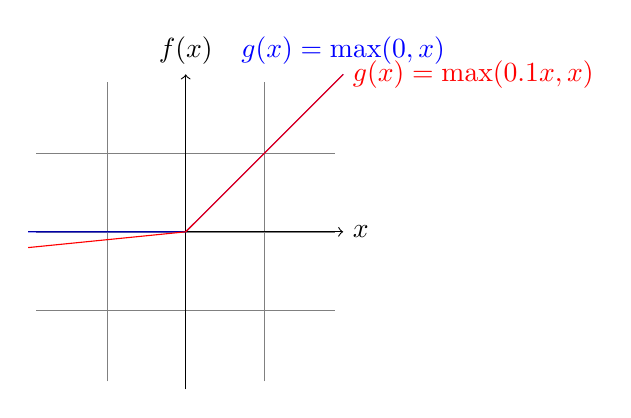
\begin{tikzpicture}[domain=-2:2]
    \draw[very thin,color=gray] (-1.9, -1.9) grid (1.9, 1.9);
    \draw[->] (-2,0) -- (2,0) node[right] {$x$};
    \draw[->] (0,-2) -- (0,2) node[above] {$f(x)$};
    \draw[color=blue]	plot (\x,{max(0, \x)})					node[above] {$g(x) = \max(0, x)$};
    \draw[color=red]	plot (\x,{max(0.1 * \x, \x)})			node[right] {$g(x) = \max(0.1x, x)$};
\end{tikzpicture}

\subsubsection{ReLU}
\begin{equation}
    g(x) = \max(0, x)
\end{equation}

\subsubsection{Leaky ReLU}
\begin{equation}
    g(x) = \max(0.01x, x)
\end{equation}

\subsubsection{PReLU}
\begin{equation}
    g(x) = \max(\alpha x, x)
\end{equation}

\subsection{haha}
\begin{tikzpicture}[domain=-2:2]
    \draw[very thin,color=gray] (-1.9, -1.9) grid (1.9, 1.9);
    \draw[->] (-2,0) -- (2,0) node[right] {$x$};
    \draw[->] (0,-2) -- (0,2) node[above] {$f(x)$};
    \draw[color=blue]	plot (\x,{tanh(\x) + 0.25 * \x})					node[right] {$g(x) = \tanh(x) + 0.25x$};
\end{tikzpicture}

\begin{equation}
    \begin{split}
        g(x) &= \tanh(x) + 0.25x \\
        g(x)' &= 0.75 - g(x)^2 \\ &= 0.75 - \tanh(x)^2
    \end{split}
\end{equation}

\subsection{Loss functions}



\section{信息熵}
\subsection{信息量}
信息量和具体的事件相关,且越小概率的事件发生产生的信息量越大。因此,\textbf{一个具体事件的信息量应该是随着其发生概率而递减的,且不能为负}。
如果我们有俩个不相关的事件x和y,那么我们观察到的俩个\textbf{独立事件同时发生时获得的信息应该等于观察到的事件各自发生时获得的信息之和},即为:
\begin{equation}
    \begin{split}
        h(x, y) &= h(x) + h(y) \\
        p(x, y) &= p(x) + p(y)
    \end{split}
\end{equation}
为满足以上性质,信息量$h(x)$公式为下
\begin{equation}
    h(x) = -\log_2p(x)
\end{equation}
\subsection{信息熵}
信息熵即为随机变量的信息量的期望
\begin{equation}
    H(x) = -\sum_ip(x_i)\log_2p(x_i)
\end{equation}
\subsection{条件熵}
\begin{equation}
    H(X|Y) = -\sum_{i,j}p(x_i, y_j)\log \frac{p(x_i, y_i)}{p(y_i)}
\end{equation}

\subsection{Mutual Information}
互信息是衡量随机变量之间互相依赖程度的度量。
\begin{equation}
    \begin{split}
        I(X;Y) &= H(X) - H(X|Y) \\
        &=\sum_y\sum_x p(x, y)\log(\frac{p(x, y)}{p(x)p(y)})
    \end{split}
\end{equation}

\section{Batch Normalization}
机器学习中假设:源空间和目标空间的数据分布是一致的,如果不一致,就是新的机器学习问题,例如transfer learning/domain adaptation
等。而covariate shift就是分布不一致假设下的一个分支问题,它指的是源空间和目标空间的条件概率是一致的,但是其边缘概率不同.
对于所有$x \in \chi $
\begin{equation}
    \begin{split}
        P_s(Y|X = x) &= P_t(Y|X = x) \\
        P_s(X) &\neq P_t(X)
    \end{split}
\end{equation}
\begin{quotation}
    \textbf{Internal Covariate Shift} Training Deep Neural Networks is complicated by the fact that the distribution of each layer's inputs
changes during training, as the parameters of the previous layers change. And this slows down the training 
by requring lower lr ant careful parameter initialization, and makes it notoriously hard to train models
with saturating nonlinearities.
\end{quotation}
解决方案:白化操作可以使得数据变为\textbf{独立同分布}
\begin{quotation}
    By whitening the inputs to each layer, we would take a step towards achieving the fixed distribution
    of inputs that would remove the ill effects of the ICS.
\end{quotation}
但是每层的白化会影响梯度下降优化过程。每层进行白化计算量过大。保证模型的表达能力不因为规范化而下降。 

Simply normalizaing each input of a layer may change what the layer can represent. So, we make sure that
the transformation inserted in the network can represent the identity transform.
\begin{figure}[H]
    \centering
    \includegraphics[width=8.5cm]{images/bn_algorithm.png}
    \caption{Batch Normalization}
    \label{fig:batchnorm}
\end{figure}

\section{How Does Batch Normalization Help Optimization?}
Batch Normalization 对减少ICS起到了很少的作用,it makes the optimization landscape significantly smoother.
\begin{itemize}
    \item \textbf{Is the effectiveness of BatchNorm indeed related to internal covariate shift?} The 'noisy' BatchNorm 
    network has qualitatively less stable distributions than even the standard, non-BatchNoram network, yet it still 
    better performs better in terms of training.
    \item \textbf{Is BatchNorm reducing internal covariate shift?} We Observe that networks with BatchNorm often
    exhibit an increase in ICS.
\end{itemize}
\begin{figure}[H]
    \centering
    \includegraphics[width=14cm]{images/bn_landscape.png}
    \label{fig:bn_landscape}
\end{figure}

\textbf{Why does BatchNorm work?}


BatchNorm reparametrizes the underlying optimization problem to make its landscape significatly more smooth.
The key implication of BatchNorm's reparametrization is that it makes the gradients more reliable and predictive.
After all, improved Lipschitzness of the gradients gives us confidence that when we take a larger step in a direction 
of a computed gradient, this gradient direction remains a fairly accurate estimate of the actual gradient direction after 
taking that step.

\textbf{Is BatchNorm the best way to smoothen the landscape?}

In fact, for deep linear networks, $l_1$–normalization performs even better than BatchNorm. Note that, 
qualitatively, the $l_p$–normalization techniques lead to larger distributional shift than the vanilla,
 i.e., unnormalized, networks, yet they still yield improved optimization performance.